\beginsong{Il canto della promessa}

\begin{tikzpicture}[remember picture, overlay]
    \node[inner sep=0pt, anchor=south east] 
    at ([yshift=0.7cm]current page text area.south east) { % Centra l'immagine nella pagina
        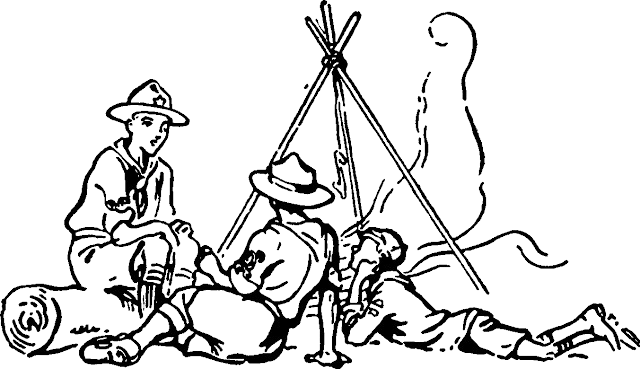
\includegraphics[width=0.8\paperwidth]{img/promessa.png} 
    };
\end{tikzpicture}

\begin{tikzpicture}[remember picture, overlay]
    \node[inner sep=0pt, anchor=north east] 
    at ([yshift=-0.7cm]current page text area.north east) { % Centra l'immagine nella pagina
        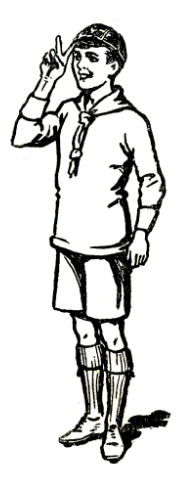
\includegraphics[width=0.12\paperwidth]{img/saluto.png} 
    };
\end{tikzpicture}

\beginverse

\[RE]Dinnanzi a voi mi impegno 
sul mio on\[LA7]or 
e \[RE]voglio esserne degno 
per \[LA7]Te o Signor

\endverse

\beginchorus

La \[SOL]giusta e retta \[RE]via, \[LA7]mostrami \[RE]tu 
e \[SOL]la promessa \[RE]mia, \[LA7]accogli o \[RE]Gesù 

\endchorus

\chordsoff

\beginverse

Leale alla mia legge, sempre sarò 
se la Tua man mi regge, io manterrò 

\endverse

\beginchorus

La giusta e retta via \dots

\endchorus

\endsong